% =====================================================================
%  AetherGrid AI: System Design Report
%  Document AEG-RPT-001, Rev 0.1.0, Draft for Design Review
%  Compile: pdflatex main.tex (twice)
% =====================================================================
\documentclass[11pt,a4paper]{article}

\usepackage[T1]{fontenc}
\usepackage[utf8]{inputenc}
\usepackage{mathpazo}
\usepackage{helvet}
\usepackage{courier}
\usepackage{microtype}
\usepackage[margin=2.6cm,headheight=14pt]{geometry}
\usepackage{xcolor}
\usepackage{titlesec}
\usepackage{fancyhdr}
\usepackage{lastpage}
\usepackage{booktabs}
\usepackage{array}
\usepackage{enumitem}
\usepackage{amsmath,amssymb,amsthm}
\usepackage{tcolorbox}
\usepackage{float}
\usepackage{caption}
\usepackage{tikz}
\usetikzlibrary{arrows.meta,positioning,calc}
\usepackage{pgfplots}
\pgfplotsset{compat=1.18}
\usepackage{hyperref}

% Palette: botanical / heritage
\definecolor{navy}{HTML}{2F5233}       % deep forest green
\definecolor{steel}{HTML}{B07D32}      % warm amber
\definecolor{brick}{HTML}{A14523}      % muted clay
\definecolor{rulegray}{HTML}{B5A99A}   % warm stone
\definecolor{lightfill}{HTML}{F4EFE5}  % warm cream

% Typography and global spacing
\renewcommand{\familydefault}{\rmdefault}
\setlength{\parindent}{0pt}
\setlength{\parskip}{8pt}
\renewcommand{\arraystretch}{1.25}      % roomier table rows
\setlength{\intextsep}{14pt}            % space above/below [H] floats

\titleformat{\section}
  {\Large\sffamily\bfseries\color{navy}}
  {\thesection}{0.9em}{}
  [\vspace{2pt}{\color{navy}\titlerule[1.2pt]}]
\titleformat{\subsection}
  {\large\sffamily\bfseries\color{navy!90!black}}
  {\thesubsection}{0.8em}{}
\titleformat{\subsubsection}
  {\sffamily\bfseries\color{black}}
  {\thesubsubsection}{0.7em}{}
\titlespacing*{\section}{0pt}{14pt}{12pt}
\titlespacing*{\subsection}{0pt}{10pt}{6pt}

% Formal environments with generous spacing so each block breathes
\newtheoremstyle{spaceddef}{14pt}{14pt}{}{}{\bfseries\sffamily}{.}{0.8em}{}
\newtheoremstyle{spacedplain}{14pt}{14pt}{\itshape}{}{\bfseries\sffamily}{.}{0.8em}{}
\theoremstyle{spaceddef}
\newtheorem{definition}{Definition}[section]
\newtheorem{assumption}{Assumption}[section]
\theoremstyle{spacedplain}
\newtheorem{proposition}{Proposition}[section]
\newtheorem{property}{Property}[section]
\newtheorem{hypothesis}{Hypothesis}[section]

\newtcolorbox{statement}[1]{colback=lightfill,colframe=navy,boxrule=.5pt,
  arc=1pt,left=11pt,right=11pt,top=9pt,bottom=9pt,title={#1},
  fonttitle=\sffamily\small\bfseries,coltitle=white,
  colbacktitle=navy,toptitle=6pt,bottomtitle=6pt}

% Headers and footers
\pagestyle{fancy}
\fancyhf{}
\fancyhead[L]{\sffamily\small\color{navy}AetherGrid AI: System Design Report}
\fancyhead[R]{\sffamily\small AEG-RPT-001 \,$\cdot$\, Rev 0.1.0}
\fancyfoot[L]{\sffamily\footnotesize\color{black!60}Internal, for design review}
\fancyfoot[C]{\sffamily\small Page \thepage\ of \pageref{LastPage}}
\fancyfoot[R]{\sffamily\footnotesize\color{black!60}Aug 2026}
\renewcommand{\headrulewidth}{0.5pt}
\renewcommand{\headrule}{\hbox to\headwidth{\color{rulegray}\leaders\hrule height .5pt\hfill}}
\fancypagestyle{plain}{\fancyhf{}\fancyfoot[C]{\sffamily\small Page \thepage\ of \pageref{LastPage}}
  \renewcommand{\headrule}{}}

\captionsetup{font=small,labelfont={bf,sf,color=navy},skip=10pt}
\hypersetup{colorlinks=true,linkcolor=navy,urlcolor=navy,citecolor=navy,
  pdftitle={AetherGrid AI: System Design Report AEG-RPT-001}}

\begin{document}

% =====================================================================
%  COVER PAGE
% =====================================================================
\begin{titlepage}
\thispagestyle{empty}
{\sffamily
\begin{tabular*}{\textwidth}{@{}l@{\extracolsep{\fill}}r@{}}
\textbf{\color{navy}AETHERGRID PROGRAMME} & \textbf{AEG-RPT-001} \\
\end{tabular*}}
\par\vspace{2pt}{\color{navy}\rule{\textwidth}{1.2pt}}

\vspace*{3.2cm}
\begin{center}
{\sffamily\small\color{black!60}SYSTEM DESIGN REPORT\par}
\vspace{0.9cm}
{\sffamily\Huge\bfseries\color{navy} AetherGrid AI\par}
\vspace{0.6cm}
{\Large Autonomous Multi-Agent Logistics and\\[2pt] Emergency Dispatch Simulation\par}
\vspace{1.2cm}
{\color{rulegray}\rule{0.55\textwidth}{0.6pt}}
\end{center}

\vspace{1.6cm}
{\small
\begin{tabular*}{\textwidth}{@{}>{\sffamily\bfseries}p{4.2cm}@{\extracolsep{\fill}}p{9.5cm}@{}}
\toprule
Document no.   & AEG-RPT-001 \\
Status         & Draft for design review \\
Prepared by    & Design Engineering \\
Review panel   & To be assigned at design review \\
\bottomrule
\end{tabular*}}

\vspace{1.4cm}
{\small
\begin{tabular*}{\textwidth}{@{}>{\sffamily\bfseries}p{4.2cm}@{\extracolsep{\fill}}p{3.2cm}p{3.2cm}p{2.6cm}@{}}
\toprule
Role & Name & Roll Number: \\
\midrule
Author 1 & Sparsh Verma  & 1024240011 \\
Author 2 & Vishal Singla & 1024240009 \\
\bottomrule
\end{tabular*}}

\vfill
{\footnotesize\color{black!60}
\textbf{Revision history.}\quad
Rev 0.1.0: initial draft issued for design review. All quantitative figures are
design projections; no empirical results are reported (see \S1.4).\par}
\end{titlepage}

% =====================================================================
%  FRONT MATTER
% =====================================================================
\tableofcontents
\listoffigures
\listoftables
\newpage

\section{Introduction}

\subsection{Purpose and scope}
This report sets out the design of \textbf{AetherGrid AI}, a discrete-event
simulation engine and mission-control platform for autonomous fleet routing,
emergency triage dispatch, dynamic pathfinding, and reinforcement-learning (RL)
fleet re-positioning. Section~\ref{sec:problem} formulates the problem,
\S\ref{sec:arch} describes the architecture, \S\ref{sec:sim} the simulation
model, \S\ref{sec:algo} the algorithmic framework, \S\ref{sec:hmi} the
mission-control interface, \S\ref{sec:vv} verification and validation, and
\S\ref{sec:plan} the implementation plan.

\subsection{Design tenets}
Four principles shape the design:
\begin{enumerate}[leftmargin=1.6em,itemsep=2pt]
  \item \textbf{Determinism.} A fixed seed produces a byte-identical metric log,
        verified by SHA-256, so every experiment in \S\ref{sec:vv} can be repeated exactly.
  \item \textbf{Pluggability.} Dispatch and routing strategies are runtime callbacks.
        Any of them can be swapped without touching the engine.
  \item \textbf{Lean runtime.} Python standard library plus NumPy, in an isolated
        \texttt{venv}. No frameworks.
  \item \textbf{Unit consistency.} Every cost in the system is expressed in seconds,
        which lets distance, congestion, weather and deadlines be compared directly.
\end{enumerate}

\subsection{Definitions and abbreviations}
\begin{table}[H]\centering\small
\begin{tabular}{@{}>{\bfseries}l@{\hspace{1.5em}}p{9.5cm}@{}}
\toprule
ETA & Estimated time of arrival (shortest-path cost on the priced graph) \\
SLA & Service-level agreement; maximum admissible response time \\
VRPTW & Vehicle routing problem with time windows \\
FSM & Finite-state machine \\
EWMA & Exponentially weighted moving average \\
RL & Reinforcement learning \\
\bottomrule
\end{tabular}
\caption{Abbreviations used in this document.}
\end{table}

\subsection{Statement on data provenance}
\begin{statement}{Data provenance}
AetherGrid AI has not been implemented yet, so this report contains no
measurements. Figures labelled \emph{projected} are design projections, used only
to size the Phase 4 benchmark (\S\ref{sec:bench}). The empirical commitments of
the project are the three pre-registered hypotheses in \S\ref{sec:hyp}, each
written down with its test protocol and falsification condition before any data
exist. If the data falsify a hypothesis, that counts as a valid result.
\end{statement}

\subsection{Document family and evolution}
This report is revision 0.1.0 of the system-level design baseline, not the final
word. Detailed design, implementation and validation will land as separate
controlled documents, and measured results will replace every figure currently
marked \emph{projected}.

\begin{table}[H]\centering\small
\begin{tabular}{@{}llll@{}}
\toprule
\textsc{ID} & \textsc{Document} & \textsc{Stage} & \textsc{Status} \\
\midrule
AEG-RPT-001 & System Design Report (this document) & Design review & Rev 0.1.0 draft \\
AEG-DDS-001 & Detailed design: core simulation & Phase A & Planned \\
AEG-DDS-002 & Detailed design: AI suite (routing, dispatch, RL) & Phase B & Planned \\
AEG-DDS-003 & Detailed design: mission control & Phase C & Planned \\
AEG-VER-001 & Verification plan and results (Hypotheses~\ref{hyp:1}--\ref{hyp:3}) & Phase D & Planned \\
\bottomrule
\end{tabular}
\caption{Document family. Child documents inherit the definitions, assumptions
and invariants of this baseline. Later revisions are recorded on the cover page.}
\end{table}

% =====================================================================
\section{Problem Formulation}\label{sec:problem}

\begin{definition}[Dynamic transportation network]\label{def:network}
At time $t$ the city is a directed graph $G_t=(V,E_t)$, $E_t\subseteq V\times V$.
Each edge $e$ carries length $\ell_e$, terrain class $\tau_e\ge1$, congestion
density $\rho_e(t)\in[0,1]$ (EWMA of occupancy), a weather multiplier $\omega(t)\ge1$,
and a hazard indicator. A \emph{closure} removes $e$ from $E_t$; a \emph{hazard}
retains $e$ at increased cost.
\end{definition}

\begin{definition}[Fleet]
A set $\mathcal{A}$ of heterogeneous agents (ambulance, fire engine, police, drone,
delivery van). Agent $a$ has position $\mathrm{pos}_a(t)$, battery $B_a(t)\in[0,1]$,
capacity, and status in \{\textsc{idle}, \textsc{enroute}, \textsc{servicing},
\textsc{recharging}\}.
\end{definition}

\begin{definition}[Demand process]
Calls arrive as a marked Poisson process $N(t)\sim\mathrm{Poisson}(\lambda t)$ with
diurnal rate $\lambda(t)$; call $j$ is the tuple $(\mathrm{loc}_j,\,w_j,\,D_j,\,
\text{category})$ with priority weight $w_j$, arrival deadline $D_j$, and
log-normal service time.
\end{definition}

\begin{definition}[Dispatch policy]
Every batch window $\Delta$, a policy $\pi$ maps the buffered calls $B(t)$, the
idle agents $I(t)$ and the network state $G_t$ to an assignment
$x\in\{0,1\}^{I\times B}$. Assigned agents follow least-cost paths; unassigned
calls stay in $B(t)$; idle agents may be relocated by a re-positioning policy
between windows.
\end{definition}

\paragraph{Objective.} Minimise expected weighted response $\mathbb{E}\bigl[\sum_j w_j T_j\bigr]$
subject to SLA fulfilment $P(T_j\le D_j)$ at the required levels, with online,
non-clairvoyant information.

\begin{proposition}[Complexity]\label{prop:complexity}
For $m$ idle agents and $n$ buffered calls, exhaustive assignment evaluates
$m^{n}$ candidates ($20^{12}\approx4.09\times10^{15}$ at fleet scale). The
Hungarian method recovers the exact optimum in $O(n^{3})$ \cite{kuhn1955}. When each
cost entry is a shortest path on $G_t$, the per-batch work is dominated by
$|I|\cdot|B|$ shortest-path queries. Multi-stop logistics adds per-vehicle stop
sequencing (VRPTW), which is NP-hard \cite{solomon1987}.
\end{proposition}

Exhaustive search is therefore out of the question, and the design uses layered
structure instead: a pricing layer (\S\ref{sec:cost}), an exact assignment layer
(\S\ref{sec:assign}), and a learned pre-positioning layer (\S\ref{sec:rl}).

% =====================================================================
\section{System Architecture}\label{sec:arch}

\subsection{Topology}
\begin{figure}[H]\centering
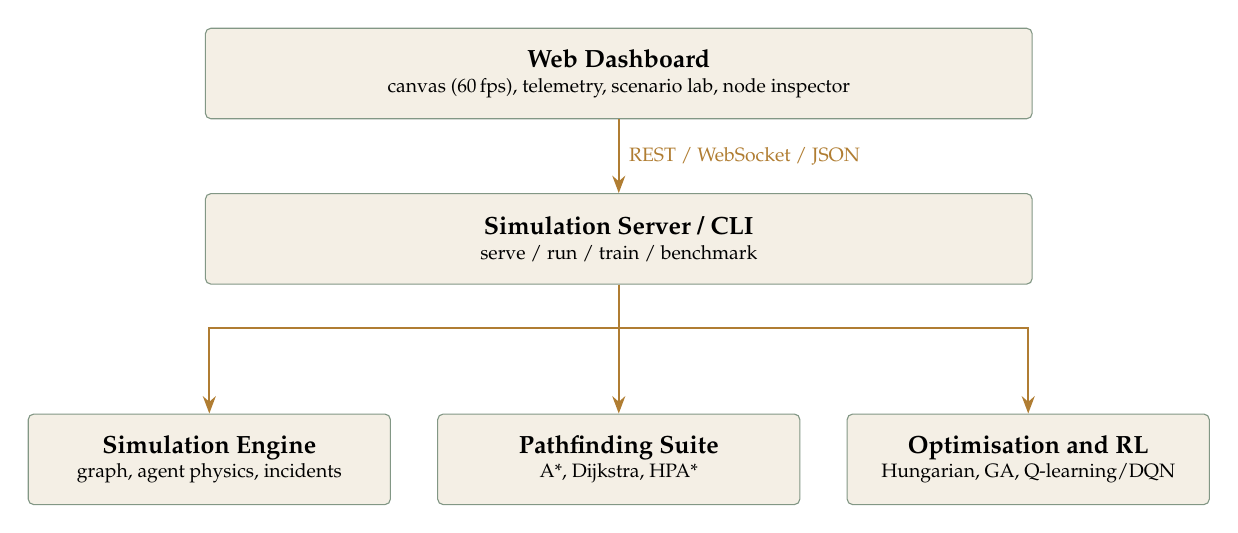
\begin{tikzpicture}[
  box/.style={draw=navy!60,fill=lightfill,rounded corners=2pt,
              minimum width=4.6cm,minimum height=1.15cm,align=center,font=\small},
  big/.style={box,minimum width=10.5cm},
  arr/.style={-{Stealth[length=2.2mm]},steel,thick}]
\node[big] (web) at (0,0) {\textbf{Web Dashboard}\\[-2pt]{\scriptsize canvas (60\,fps), telemetry, scenario lab, node inspector}};
\node[big] (srv) at (0,-2.1) {\textbf{Simulation Server / CLI}\\[-2pt]{\scriptsize serve / run / train / benchmark}};
\node[box] (eng) at (-5.2,-4.9) {\textbf{Simulation Engine}\\[-2pt]{\scriptsize graph, agent physics, incidents}};
\node[box] (pf)  at (0,-4.9)   {\textbf{Pathfinding Suite}\\[-2pt]{\scriptsize A*, Dijkstra, HPA*}};
\node[box] (opt) at (5.2,-4.9) {\textbf{Optimisation and RL}\\[-2pt]{\scriptsize Hungarian, GA, Q-learning/DQN}};
\draw[arr] (web) -- node[right,font=\scriptsize\color{steel}]{REST / WebSocket / JSON} (srv);
\draw[arr] (srv.south) -- ++(0,-0.55) -| (eng);
\draw[arr] (srv) -- (pf);
\draw[arr] (srv.south) -- ++(0,-0.55) -| (opt);
\end{tikzpicture}
\caption{System topology. Dispatch strategies are injected as callbacks; the engine
runs identically headless (CI) or attached to the dashboard.}
\label{fig:arch}
\end{figure}

\subsection{Component responsibilities}
\begin{table}[H]\centering\small
\begin{tabular}{@{}>{\sffamily\bfseries}l@{\hspace{1em}}p{7.6cm}l@{}}
\toprule
Module & Responsibility & Path \\
\midrule
Simulation Engine & graph, agent FSM and physics, Poisson generator, event loop & \texttt{core/} \\
Pathfinding Suite & dynamic A*, Dijkstra ETA matrices, hierarchical HPA* & \texttt{ai/pathfinding.py} \\
Dispatchers & greedy baseline, Hungarian matcher, genetic VRPTW & \texttt{ai/dispatchers.py} \\
RL Core & Q-learning $\rightarrow$ DQN idle re-positioning & \texttt{ai/rl\_agent.py} \\
Mission Control & HTTP/WS server, canvas visualiser, telemetry, scenario lab & \texttt{web/} \\
\bottomrule
\end{tabular}
\caption{Component responsibilities and repository mapping.}
\end{table}

\subsection{Interfaces and determinism}
The dashboard receives state diffs at 10\,Hz and interpolates them to 60\,fps.
Commands flow the other way: inject hazard, close edge, set weather, switch
strategy. All randomness passes through a single seeded generator
(Assumption~\ref{assum:det}).

\begin{assumption}[Determinism]\label{assum:det}
With a fixed seed, the sequence of arrivals, service times and tie-breaks is
reproduced exactly; metric logs are byte-identical across runs.
\end{assumption}

\subsection{Dependency policy}
The runtime is stdlib plus NumPy. We hand-roll the web layer over HTTP/WebSocket
rather than adopting a framework, and the engine is importable, so tests,
notebooks and the server all embed the same \texttt{SimulationEngine}.

% =====================================================================
\section{Simulation Model}\label{sec:sim}

\subsection{Environment coefficients}
\begin{table}[H]\centering\small
\begin{tabular}{@{}lr@{\hspace{3em}}lr@{}}
\toprule
\textsc{Terrain} & $\tau_e$ & \textsc{Weather} & $\omega(t)$ \\
\midrule
Highway  & \textbf{1.00} & Clear & \textbf{1.00} \\
Arterial & 1.25          & Rain  & 1.22 \\
Urban    & 1.45          & Fog   & 1.45 \\
Alley    & 1.90          & Snow  & 1.85 \\
Offroad  & 3.10          &       &      \\
\bottomrule
\end{tabular}
\caption{Travel-time multipliers. Defaults: $\alpha=0.85$, $\beta=45$\,s.}
\label{tab:env}
\end{table}

\begin{statement}{Closure vs.\ hazard (normative)}
A \textbf{closed} edge is removed from $E_t$ and must force re-routing; a
\textbf{hazard} remains traversable at penalty $\beta$. Implementations must not
conflate the two: the distinction matters for admissibility
(Property~\ref{prop:admiss}) and for invariant I5 (\S\ref{sec:inv}).
\end{statement}

\subsection{Agent dynamics}
Battery evolves as
\begin{equation}
B_a(t+\Delta t)=B_a(t)-\Delta t\,\bigl(p_0+p_1\,v\,\mathrm{load}\bigr)/E_{\mathrm{cap}},
\end{equation}
with logistic charging. Emergency agents apply siren mode (congestion weight
$\times0.35$) and priority escalation ($w_j\mathrel{+}=0.2$ per minute of SLA
excess); logistics agents run capacity-constrained multi-drop routes.

\begin{figure}[H]\centering
\begin{tikzpicture}[
  st/.style={draw=#1,fill=#1!6,rounded corners=3pt,minimum width=2.7cm,
             minimum height=.95cm,font=\small\bfseries\sffamily,text=#1},
  st/.default=navy,
  arr/.style={-{Stealth[length=2.2mm]},steel,thick}]
\node[st]        (I) at (0,0)    {IDLE};
\node[st=brick]  (E) at (4,1.6)  {ENROUTE};
\node[st=brick!70](S) at (8,0)   {SERVICING};
\node[st=steel]  (R) at (4,-1.8) {RECHARGING};
\draw[arr] (I) to[bend left=18] node[above,font=\scriptsize]{dispatch} (E);
\draw[arr] (E) to[bend left=18] node[above,font=\scriptsize]{arrival} (S);
\draw[arr] (S) to[bend left=18] node[below,font=\scriptsize]{complete} (I);
\draw[arr] (I) to[bend right=22] node[left,font=\scriptsize]{$B<20\%$} (R);
\draw[arr] (R) to[bend right=22] node[right,font=\scriptsize]{$B\ge90\%$} (I);
\draw[arr,dashed] (E) to[bend right=14] node[right,font=\scriptsize]{$B<12\%$ (preempt)} (R);
\end{tikzpicture}
\caption{Agent finite-state machine. Transitions are asserted at step boundaries (I2, I6).}
\label{fig:fsm}
\end{figure}

\subsection{Incident model}
Inter-arrival times are $\mathrm{Exp}(\lambda)$; the diurnal schedule (Figure~\ref{fig:lambda})
applies rush multipliers of $2.4\lambda_0$.

\begin{figure}[H]\centering
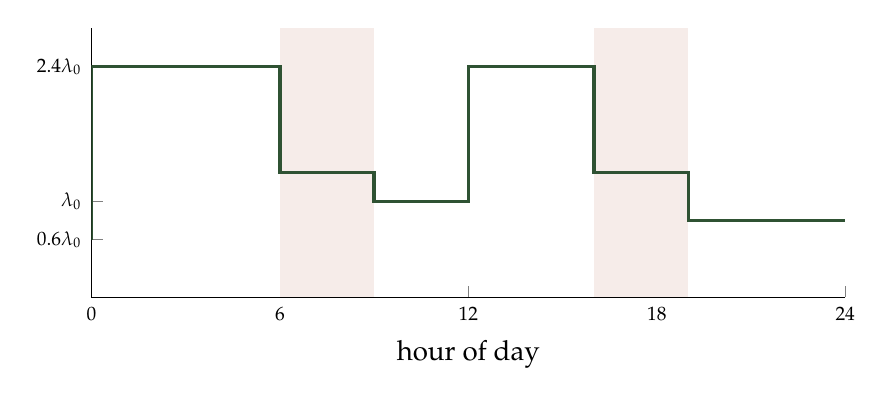
\begin{tikzpicture}
\begin{axis}[width=.92\linewidth,height=5cm,xmin=0,xmax=24,ymin=0,ymax=2.8,
  axis lines*=left,xtick={0,6,12,18,24},ytick={0.6,1,2.4},
  yticklabels={$0.6\lambda_0$,$\lambda_0$,$2.4\lambda_0$},
  tick label style={font=\scriptsize},xlabel={hour of day}]
  \fill[brick!10] (axis cs:6,0) rectangle (axis cs:9,2.8);
  \fill[brick!10] (axis cs:16,0) rectangle (axis cs:19,2.8);
  \addplot[navy,const plot mark right,line width=1.2pt] coordinates
    {(0,0.6)(6,2.4)(9,1.3)(12,1.0)(16,2.4)(19,1.3)(22,0.8)(24,0.8)};
\end{axis}
\end{tikzpicture}
\caption{Diurnal arrival-rate schedule $\lambda(t)$ (design parameter).}
\label{fig:lambda}
\end{figure}

\begin{table}[H]\centering\small
\begin{tabular}{@{}lclll@{}}
\toprule
\textsc{Category} & $w_j$ & \textsc{Deadline} & \textsc{Service} & \textsc{Notes} \\
\midrule
Emergency medical & \textbf{1.00} & $\le 8$ min & 6--12 min & escalation on breach \\
Structure fire    & 0.90 & $\le 10$ min & 15--25 min & fire engine required \\
Hazmat            & 0.95 & $\le 12$ min & 20 min & corridor exclusion \\
Package delivery  & 0.40 & [earliest, due] & 2--4 min & soft window \\
\bottomrule
\end{tabular}
\caption{Incident taxonomy and SLA contract. Breaches are logged, never discarded.}
\end{table}

Queue diagnostics use Little's law $L=\lambda W$ \cite{little1961}, reported per zone.

% =====================================================================
\section{Algorithmic Framework}\label{sec:algo}

\subsection{Edge cost model}\label{sec:cost}
\begin{definition}[Edge cost]\label{def:cost}
\begin{equation}\label{eq:cost}
c(e,t)=\ell_e\,\tau_e\bigl(1+\alpha\,\rho_e(t)\bigr)\,\omega(t)
+\beta\,\mathbf{1}[\mathrm{hazard}_e],
\end{equation}
where $\ell_e$ is free-flow traversal time. Terrain, congestion and weather enter
multiplicatively; hazards additively; closures remove the edge (\S4.1).
\end{definition}
Everything downstream sees only $c(e,t)$. No component inspects raw map state.

\subsection{Pathfinding}
Live dispatch runs on A* with the heuristic below. The Hungarian matcher reads
cached Dijkstra distance matrices, recomputed only when the topology changes.
Long-haul queries use HPA* with precomputed boundary graphs over $8\times8$
chunks \cite{botea2004}.

\begin{property}[Admissibility]\label{prop:admiss}
With $h(n)=\tau_{\min}\cdot d(n,\mathrm{goal})$ and $\tau_e,\omega\ge1$, $h$ never
overestimates residual cost, so A* returns optimal paths on the priced graph
\cite{hart1968}. Hazmat injections raise $\beta$ without removing edges, preserving
this property.
\end{property}

\begin{figure}[H]\centering
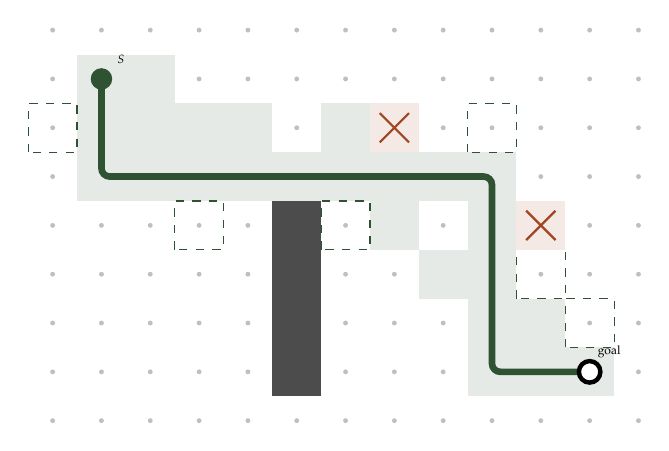
\begin{tikzpicture}[scale=0.62,transform shape]
  \foreach \x in {0,...,12}\foreach \y in {0,...,8}
    \fill[black!25] (\x+.5,\y+.5) circle (0.05);
  \foreach \x/\y in {1/7,1/6,2/6,2/7,1/5,2/5,3/5,3/6,4/5,4/6,5/5,6/5,6/6,7/5,7/4,
                     8/5,9/5,9/4,9/3,8/3,9/2,10/2,9/1,10/1,11/1}
    \fill[navy!12] (\x,\y) rectangle ++(1,1);
  \foreach \x/\y in {0/6,3/4,6/4,10/3,9/6,11/2}
    \draw[navy,dashed] (\x,\y) rectangle ++(1,1);
  \foreach \x/\y in {5/1,5/2,5/3,5/4}
    \fill[black!70] (\x,\y) rectangle ++(1,1);
  \foreach \x/\y in {7/6,10/4}{
    \fill[brick!12] (\x,\y) rectangle ++(1,1);
    \draw[brick,thick] (\x+.2,\y+.2)--(\x+.8,\y+.8) (\x+.8,\y+.2)--(\x+.2,\y+.8);}
  \draw[navy,line width=2.4pt,rounded corners=3pt]
    (1.5,7.5)--(1.5,5.5)--(9.5,5.5)--(9.5,1.5)--(11.5,1.5);
  \fill[navy] (1.5,7.5) circle (.22);
  \draw[black,fill=white,line width=1.6pt] (11.5,1.5) circle (.22);
  \node[font=\scriptsize] at (1.9,7.9) {$S$};
  \node[font=\scriptsize] at (11.9,1.9) {goal};
\end{tikzpicture}
\caption{Worked routing example: the wall forces a detour; hazards raise cost without
blocking. Shaded: closed set; dashed: open frontier.}
\label{fig:astar}
\end{figure}

\subsection{Assignment model}\label{sec:assign}
\begin{definition}[Batch assignment]\label{def:assign}
Every $\Delta=5$\,s, solve
\begin{equation}\label{eq:ilp}
\min_{x}\ \sum_{i}\sum_{j} c_{ij}x_{ij}\quad\text{s.t.}\quad
\sum_j x_{ij}\le1\ \forall i,\qquad \sum_i x_{ij}\le1\ \forall j,\qquad x\in\{0,1\},
\end{equation}
\begin{equation}\label{eq:costij}
c_{ij}=\mathrm{ETA}_{ij}+\mu\max\bigl(0,\ t+\mathrm{ETA}_{ij}-D_j\bigr),\qquad
\mathrm{ETA}_{ij}=\mathrm{dist}_{c(t)}(\mathrm{pos}_i,\mathrm{call}_j).
\end{equation}
\end{definition}
The Hungarian method \cite{kuhn1955} gives the exact optimum. The matcher only
ever sees the cost matrix from Definition~\ref{def:cost}, never the graph itself,
which is why strategies can be hot-swapped.

\begin{property}[Always feasible]\label{prop:feasible}
Because deadline violations enter as a finite penalty $\mu$ rather than hard
constraints, \eqref{eq:ilp} stays feasible for every buffer/fleet configuration,
including demand bursts. Rectangular instances ($|B|\ne|I|$) are handled by
padding. The $\le$ constraints are deliberately loose: leftover calls re-buffer,
and leftover agents feed the policy of \S\ref{sec:rl}.
\end{property}

\subsection{Re-positioning policy (RL)}\label{sec:rl}
\begin{table}[H]\centering\small
\begin{tabular}{@{}>{\sffamily\bfseries}lp{10cm}@{}}
\toprule
State & (sector, time bin, fleet occupancy vector) \\
Action & stay; relocate to adjacent sector \\
Reward & $r=-\sum_j w_jT_j-\kappa\,\Delta E+b\,\mathbf{1}[\mathrm{SLA\ met}]$ \\
Horizon & $\gamma=0.97$; decisions every 30\,s, idle agents only \\
\bottomrule
\end{tabular}
\caption{MDP specification of the re-positioning layer.}
\end{table}

\begin{definition}[Update rule]
Q-learning \cite{watkins1992}, one-step, off-policy:
\begin{equation}\label{eq:q}
Q(s,a)\leftarrow Q(s,a)+\eta\bigl[r+\gamma\max_{a'}Q(s',a')-Q(s,a)\bigr],
\end{equation}
with learning rate $\eta\in(0,1]$ ($\eta=0.1$; $\varepsilon$-greedy exploration,
$\varepsilon:1.0\to0.05$). The tabular baseline is succeeded by DQN (replay buffer
$50\,000$, target-network sync every $1\,000$ steps). We write $\eta$ for the
learning rate because $\alpha$ is already taken in \eqref{eq:cost}.
\end{definition}

\begin{assumption}[Layer separation]\label{assum:sep}
The re-positioning policy touches only idle agents, only between batch windows,
and at sector granularity. It never overrides an active dispatch. With that
boundary in place, the assignment layer of \S\ref{sec:assign} stays exact and
unmodified.
\end{assumption}

\subsection{System composition}
The layers run as one loop per batch window (Figure~\ref{fig:loop}). The cost
field (Definition~\ref{def:cost}) is maintained continuously; the ETA matrix is
derived from it; the assignment consumes the matrix; dispatch executes; and the
RL layer relocates the idle remainder before the next window.

\begin{figure}[H]\centering
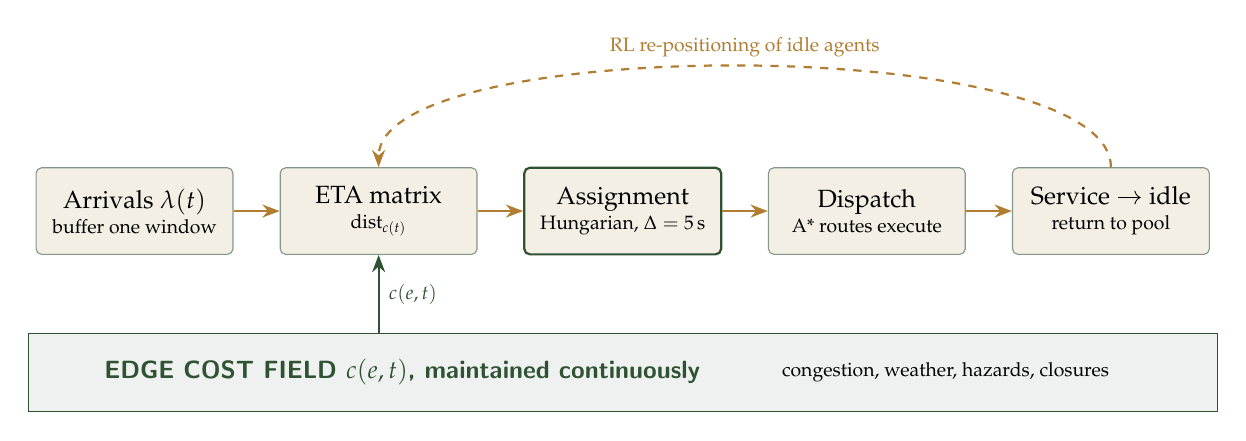
\begin{tikzpicture}[
  bx/.style={draw=navy!60,fill=lightfill,rounded corners=2pt,minimum width=2.5cm,
             minimum height=1.1cm,align=center,font=\small},
  arr/.style={-{Stealth[length=2.2mm]},steel,thick}]
\node[bx] (a) at (0,0)    {Arrivals $\lambda(t)$\\[-2pt]{\scriptsize buffer one window}};
\node[bx] (b) at (3.1,0)  {ETA matrix\\[-2pt]{\scriptsize $\mathrm{dist}_{c(t)}$}};
\node[bx,draw=navy,thick] (c) at (6.2,0) {Assignment\\[-2pt]{\scriptsize Hungarian, $\Delta=5$\,s}};
\node[bx] (d) at (9.3,0)  {Dispatch\\[-2pt]{\scriptsize A* routes execute}};
\node[bx] (e) at (12.4,0) {Service $\to$ idle\\[-2pt]{\scriptsize return to pool}};
\foreach \u/\v in {a/b,b/c,c/d,d/e}{\draw[arr] (\u) -- (\v);}
\fill[navy!8,draw=navy] (-1.35,-2.55) rectangle (13.75,-1.55);
\node[font=\small\bfseries\sffamily\color{navy}] at (3.4,-2.05)
  {EDGE COST FIELD $c(e,t)$, maintained continuously};
\node[font=\scriptsize] at (10.3,-2.05) {congestion, weather, hazards, closures};
\draw[arr,navy] (3.1,-1.55) -- (b.south) node[midway,right,font=\scriptsize\color{navy}]{$c(e,t)$};
\draw[arr,steel,dashed] (e.north) .. controls +(0,1.7) and +(0,1.7) .. (b.north)
  node[midway,above,font=\scriptsize\color{steel}]{RL re-positioning of idle agents};
\end{tikzpicture}
\caption{Per-window control loop. Every stage reads from the cost field, and the
RL layer feeds back over the idle remainder of the assignment.}
\label{fig:loop}
\end{figure}

\subsection{Compute budget}
\begin{table}[H]\centering\small
\begin{tabular}{@{}lll@{}}
\toprule
\textsc{Stage} & \textsc{Complexity} & \textsc{Notes} \\
\midrule
Cost-field update & $O(E)$ & EWMA per edge per tick \\
ETA queries & cached shortest paths & $\sim$1--2\,ms each on reference grid \\
Assignment & $O(n^{3})$ & $<2$\,ms for $n\le16$ \\
Re-positioning & $O(1)$ per idle agent & table lookup / small forward pass \\
\bottomrule
\end{tabular}
\caption{Per-window compute budget. $\Delta=5$\,s is an operational choice
(batching gain vs.\ response latency), not a compute limit.}
\end{table}

% =====================================================================
\section{Mission-Control Interface}\label{sec:hmi}
The following is to be implemented in Phase 3:
\begin{itemize}[leftmargin=1.6em,itemsep=2pt]
  \item Canvas visualisation at 60\,fps interpolated from 10\,Hz WebSocket diffs.
  \item Telemetry: response times, SLA fulfilment, battery utilisation, queue lengths.
  \item Per-node inspector exposing $c(e,t)$, $\rho_e$, $\omega$.
  \item Scenario lab: inject hazmat, induce rush-hour demand, close edges.
  \item Strategy selector for live hot-swap between dispatchers.
  \item Benchmark mode: side-by-side execution on identical seeded call streams, JSON export.
\end{itemize}

% =====================================================================
\section{Verification and Validation}\label{sec:vv}

\subsection{Pre-registered hypotheses}\label{sec:hyp}
We pre-register three hypotheses before any data exist. Directionally, we expect
$T_{\mathrm{greedy}} > T_{\mathrm{hungarian}} > T_{\mathrm{RL}}$ on mean response
time.

\begin{hypothesis}[Matching beats greedy dispatch]\label{hyp:1}
\textbf{Claim.} Under bursty demand, batch-optimal assignment yields lower mean
response time and higher SLA fulfilment than myopic nearest-unit dispatch.\\
\textbf{Test.} Seeded A/B runs with identical call streams, $\ge5$ seeds.\\
\textbf{Falsified if} no statistically significant separation is observed.
\end{hypothesis}

\begin{hypothesis}[Pre-positioning compounds]\label{hyp:2}
\textbf{Claim.} RL pre-positioning improves on assignment alone, because ETAs shrink
before matching.\\
\textbf{Test.} Hungarian vs.\ RL+Hungarian under identical seeds.\\
\textbf{Falsified if} the marginal gain $\approx0$ or the energy cost exceeds it.
\end{hypothesis}

\begin{hypothesis}[Robustness under disruption]\label{hyp:3}
\textbf{Claim.} The cost model absorbs hazards and closures: affected agents re-route
within one tick and invariants I1--I6 hold.\\
\textbf{Test.} Scenario injections mid-run with trace replay.\\
\textbf{Falsified if} re-route lags or any invariant is violated.
\end{hypothesis}

\subsection{Benchmark protocol}\label{sec:bench}
Reference scenario: $24\times24$ grid, 9 vehicles, diurnal $\lambda$ (Figure~\ref{fig:lambda}),
12\,min episodes $\times\,5$ seeds per strategy; identical call streams across
strategies; JSON reports; regressions gate merges at $\pm5\%$.

\begin{figure}[H]\centering
\begin{minipage}{0.48\linewidth}
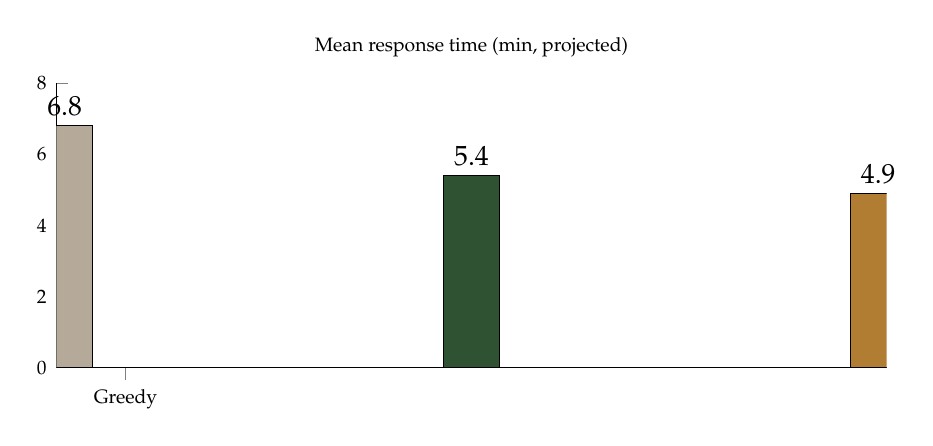
\begin{tikzpicture}\begin{axis}[ybar,bar width=20pt,width=\linewidth,height=5.2cm,
 ymin=0,ymax=8,symbolic x coords={Greedy,Hungarian,RL-Assisted},xtick=data,
 nodes near coords,nodes near coords align={vertical},axis lines*=left,
 tick label style={font=\scriptsize},title={\scriptsize Mean response time (min, projected)}]
 \addplot[fill=rulegray] coordinates {(Greedy,6.8)};
 \addplot[fill=navy]     coordinates {(Hungarian,5.4)};
 \addplot[fill=steel]    coordinates {(RL-Assisted,4.9)};
\end{axis}\end{tikzpicture}
\end{minipage}\hfill
\begin{minipage}{0.48\linewidth}
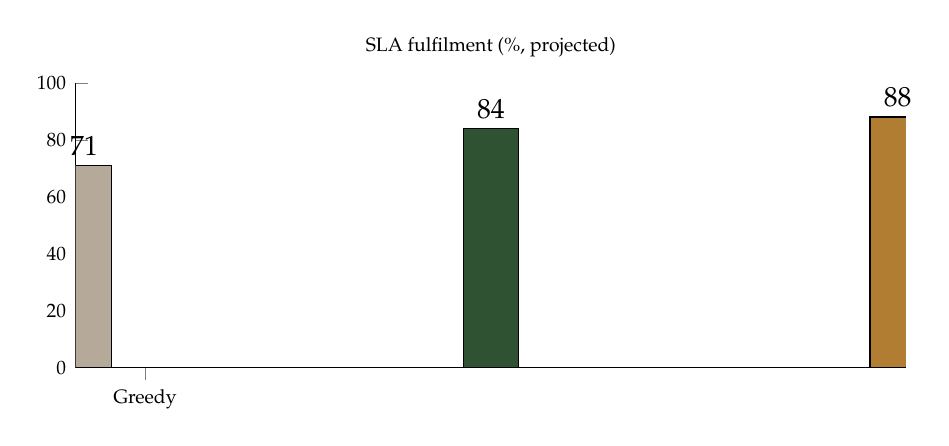
\begin{tikzpicture}\begin{axis}[ybar,bar width=20pt,width=\linewidth,height=5.2cm,
 ymin=0,ymax=100,symbolic x coords={Greedy,Hungarian,RL-Assisted},xtick=data,
 nodes near coords,nodes near coords align={vertical},axis lines*=left,
 tick label style={font=\scriptsize},title={\scriptsize SLA fulfilment (\%, projected)}]
 \addplot[fill=rulegray] coordinates {(Greedy,71)};
 \addplot[fill=navy]     coordinates {(Hungarian,84)};
 \addplot[fill=steel]    coordinates {(RL-Assisted,88)};
\end{axis}\end{tikzpicture}
\end{minipage}
\caption{Design projections used only to size the Phase 4 benchmark
(see the statement on data provenance, \S1.4).}
\label{fig:proj}
\end{figure}

\subsection{Step-boundary invariants}\label{sec:inv}
\begin{property}[Runtime invariants]\label{prop:inv}
Asserted at every simulation tick:
\begin{enumerate}[leftmargin=2em,itemsep=2pt,label=\textbf{I\arabic*.}]
  \item No agent occupies a closed edge.
  \item $B_a\in[0,1]$; charging transitions are strictly monotonic.
  \item Every completed incident carries a full path trace; SLA breaches are logged, never discarded.
  \item Identical seed $\Rightarrow$ byte-identical metric log (SHA-256).
  \item Hungarian batch cost $\le$ greedy batch cost on the same window
        (cross-validated against brute force for $n\le8$).
  \item Fleet conservation: $|\textsc{idle}|+|\textsc{enroute}|+|\textsc{servicing}|
        +|\textsc{recharging}|=|\mathcal{A}|$.
\end{enumerate}
\end{property}

\subsection{Test plan}
{\small\begin{verbatim}
# automated suite
./venv/bin/python3 -m unittest discover -s tests
# algorithm benchmark across strategies
./venv/bin/python3 -m aethergrid.cli benchmark --duration 100
# manual verification (mission control)
./venv/bin/python3 -m aethergrid.cli serve --port 8080
\end{verbatim}}
Manual checklist: zoom/pan/inspect any node; hot-swap dispatcher mid-run;
inject a closure and verify re-route within one tick.
Coverage targets: $\ge90\%$ on \texttt{core/}, $\ge85\%$ on \texttt{ai/}.

% =====================================================================
\section{Implementation Plan}\label{sec:plan}

\subsection{Phases and exit criteria}
\begin{table}[H]\centering\small
\begin{tabular}{@{}>{\sffamily\bfseries}llp{6.4cm}@{}}
\toprule
Phase & Scope & Exit criterion \\
\midrule
A & Core: grid, agents, incidents, engine & seed-stable headless run \\
B & AI suite: A*/Dijkstra/HPA*, Hungarian, GA, RL & property tests vs.\ brute force \\
C & Mission control web layer & live strategy hot-swap \\
D & Verification: benchmarks, tests, CI & Hypotheses \ref{hyp:1}--\ref{hyp:3}
      each confirmed or falsified \\
\bottomrule
\end{tabular}
\caption{Phase plan with exit criteria.}
\end{table}

\begin{figure}[H]\centering
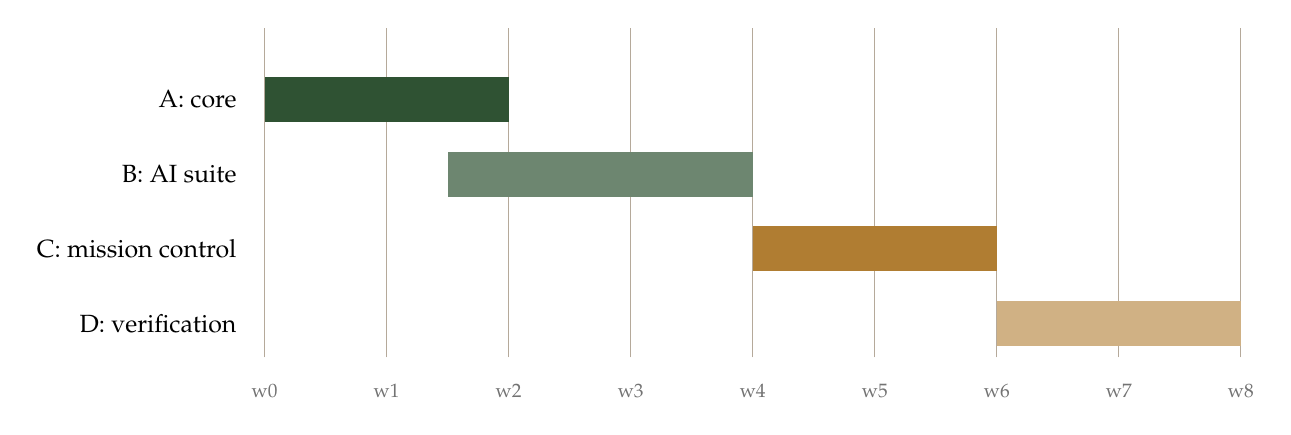
\begin{tikzpicture}[x=1.55cm,y=0.95cm,font=\small]
  \foreach \w in {0,...,8}{\draw[rulegray] (\w,0) -- (\w,4.4);
    \node[font=\scriptsize\color{black!55}] at (\w,-0.45) {w\w};}
  \fill[navy]       (0,3.15) rectangle (2,3.75);   \node[left] at (-0.15,3.45) {A: core};
  \fill[navy!70]    (1.5,2.15) rectangle (4,2.75); \node[left] at (-0.15,2.45) {B: AI suite};
  \fill[steel]      (4,1.15) rectangle (6,1.75);   \node[left] at (-0.15,1.45) {C: mission control};
  \fill[steel!60]   (6,0.15) rectangle (8,0.75);   \node[left] at (-0.15,0.45) {D: verification};
\end{tikzpicture}
\caption{Indicative schedule (weeks).}
\end{figure}

\subsection{Repository layout}
{\small\begin{verbatim}
aethergrid/
|-- core/    grid.py  agents.py  incidents.py  engine.py
|-- ai/      pathfinding.py  dispatchers.py  rl_agent.py
|-- web/     server.py  index.html  app.js  styles.css
`-- cli.py
tests/       test_simulation.py  test_pathfinding.py  test_dispatch.py
\end{verbatim}}

% =====================================================================
\section{Risks and Open Questions}
\begin{table}[H]\centering\small
\begin{tabular}{@{}p{4.4cm}llp{5.6cm}@{}}
\toprule
\textsc{Risk} & \textsc{L} & \textsc{I} & \textsc{Mitigation} \\
\midrule
RL training instability & M & M & tabular baseline first; seeded replays; fallback to static posting \\
ETA cache staleness & M & H & recompute on topology events; staleness bound asserted \\
Benchmark variance masks effects & M & M & $\ge5$ seeds; identical streams; $\pm5\%$ merge gate \\
Web-layer scope creep & H & L & spec frozen at \S\ref{sec:hmi}; deferred to Phase 3 exit \\
HPA* precompute cost & L & M & granularity sweep scheduled in Phase B \\
\bottomrule
\end{tabular}
\caption{Risk register (L = likelihood, I = impact: L/M/H).}
\end{table}
Open questions for the panel: where the knee of batch window $\Delta$ sits, what
HPA* chunk granularity to use, and whether the RL reward needs fairness terms.

% =====================================================================
\section{Conclusion}
The design splits dynamic dispatch into three layers that can each be verified on
their own: a cost field maintained continuously, an exact batch assignment over
that field, and a constrained re-positioning policy for the idle remainder.
Because the whole system is deterministic by construction, every claim made here
can be tested later. If this report is approved, we begin Phase A.

% =====================================================================
%  REFERENCES
% =====================================================================
\begin{thebibliography}{9}
\bibitem{hart1968} P.~E.~Hart, N.~J.~Nilsson, B.~Raphael. A formal basis for the
heuristic determination of minimum cost paths. \emph{IEEE Trans.\ Systems Science
and Cybernetics}, 4(2):100--107, 1968.
\bibitem{kuhn1955} H.~W.~Kuhn. The Hungarian method for the assignment problem.
\emph{Naval Research Logistics Quarterly}, 2(1--2):83--97, 1955.
\bibitem{solomon1987} M.~M.~Solomon. On the worst-case performance of some
algorithms for the vehicle routing problem with time windows.
\emph{Transportation Science}, 21(1):16--29, 1987.
\bibitem{botea2004} A.~Botea, M.~M\"uller, J.~Schaeffer. Near-optimal search with
continuous abstractions. \emph{Journal of Artificial Intelligence Research},
21:285--313, 2004.
\bibitem{watkins1992} C.~J.~C.~H.~Watkins, P.~Dayan. Q-learning.
\emph{Machine Learning}, 8:279--292, 1992.
\bibitem{little1961} J.~D.~C.~Little. A proof for the queuing formula $L=\lambda W$.
\emph{Operations Research}, 9(3):383--387, 1961.
\end{thebibliography}

% =====================================================================
%  APPENDICES
% =====================================================================
\appendix
\section{Notation}
\begin{table}[H]\centering\small
\begin{tabular}{@{}>{\centering\arraybackslash}p{2.2cm}p{5.2cm}@{\hspace{1.5em}}>{\centering\arraybackslash}p{2.2cm}p{5.2cm}@{}}
\toprule
$\ell_e$ & free-flow traversal time & $\eta$ & RL learning rate \\
$\tau_e,\ \omega$ & terrain / weather multipliers & $\gamma$ & discount factor (0.97) \\
$\rho_e(t)$ & congestion density (EWMA) & $\mu$ & deadline-penalty weight \\
$\alpha$ & congestion sensitivity (0.85) & $\Delta$ & batch window (5\,s) \\
$\beta$ & hazard penalty (45\,s) & $D_j$ & arrival deadline of call $j$ \\
\bottomrule
\end{tabular}
\caption{Principal notation.}
\end{table}

\section{Parameter Defaults}
\begin{table}[H]\centering\small
\begin{tabular}{@{}lll@{}}
\toprule
\textsc{Parameter} & \textsc{Default} & \textsc{Location} \\
\midrule
$\alpha$ (congestion sensitivity) & 0.85 & cost model \\
$\beta$ (hazard penalty) & 45\,s & cost model \\
$\Delta$ (batch window) & 5\,s & assignment \\
$\mu$ (deadline penalty) & 2.0 & assignment \\
$\gamma$ (discount) & 0.97 & RL \\
$\eta$ (learning rate) & 0.1 & RL \\
$\varepsilon$ decay & $1.0\to0.05$ over 200k steps & RL \\
Rush multiplier & $2.4\lambda_0$ & demand \\
\bottomrule
\end{tabular}
\caption{Tunable defaults (all overridable per scenario).}
\end{table}

\section{Worked Example: One Batch Window}
Three idle agents $V_1,V_2,V_3$; buffered calls $M$ (medical, $D_M=t+5$\,min) and
$F$ (fire, $D_F=t+10$\,min); $\mu=2$. ETAs (min): $M:(4.2,\,4.9,\,6.5)$,
$F:(4.6,\,8.0,\,7.2)$. Deadline pricing raises $c_{3M}=6.5+2(1.5)=9.5$; all other
entries equal their ETAs. Greedy dispatch (calls in arrival order) selects
$M\!\to\!V_1$, $F\!\to\!V_3$: total $11.4$\,min. The Hungarian optimum is
$M\!\to\!V_2$, $F\!\to\!V_1$: total $9.5$\,min ($\approx17\%$ better), leaving
$V_3$ idle. The RL layer compares $Q(\text{stay})=-12.4$ against
$Q(\text{north})=-8.1$, orders $V_3$ north, and the TD update with $\eta=0.1$,
$r=-6.0$, $\max_{a'}Q(s')=-7.5$ gives
$Q\leftarrow -8.1+0.1\bigl(-6.0+0.97(-7.5)+8.1\bigr)=-8.62$.

\end{document}
